\documentclass[a4paper,11pt]{jsarticle}

\usepackage[english]{babel}
\usepackage{amssymb, amsmath, amsthm}
\usepackage{bm}
\usepackage[dvipdfmx]{graphicx}
\usepackage{authblk}
\usepackage{indentfirst}
\usepackage{mathtools}
\usepackage{enumitem}

\theoremstyle{definition}
\newtheorem{dfn}{Definition}[section]
\newtheorem{prop}[dfn]{Proposition}
\newtheorem{lem}[dfn]{Lemma}
\newtheorem{thm}[dfn]{Theorem}
\newtheorem{cor}[dfn]{Corollary}
\newtheorem{rem}[dfn]{Remark}
\newtheorem{fact}[dfn]{Fact}

\renewcommand{\refname}{References}

% (Useful) Sets
\newcommand{\NaturalNumberSet}{\mathbb{N}}
\newcommand{\RealNumberSet}{\mathbb{R}}
\newcommand{\NDemenstionalRealEuclideanSpace}{\mathbb{R}^n}

% (Useful) Texts
\newcommand{\SuchThat}{\quad\text{s.t.}\quad}
\newcommand{\With}{\quad\text{with}\quad}

\newcommand{\Painleve}{Painlev\'e}
\newcommand{\InnerProduct}[2]{\left\langle {#1},{#2}\right\rangle} % <x,y>
\newcommand{\Norm}[1]{\left\lVert {#1} \right\rVert} % <x,y>
\newcommand{\SetValudMapping}{\it \Gamma}

\newcommand{\Closure}[1]{\text{\rm cl\:${#1}$}} % cl

% Set form e.g. {x | ...}
% #1: element
% #2: conditions
\newcommand{\SetForm}[2]{
  \{{#1}\:|\:{#2}\}
}

\SetLabelAlign{Center}{\hfil#1\hfil}
\SetLabelAlign{CenterWithParen}{\hfil(\makebox[1.0em]{#1})\hfil}

\title{%
A relation between Asymptotic Cones and \Painleve-Kuratowski Convergence \\
  \large (漸近錐と集合値写像の半連続性の関係について
  )}
\author{Ryota Iwamoto and Tamaki Tanaka}
\affil{Graduate School of Science and Technology
Niigata University}
\date{\vspace{-5ex}}

\begin{document}
\maketitle
\section{\rm Introduction}

Asymptotic cone is a significant concept in convex analysis and optimization. The asymptotic cone of a set is defined as the set of all directions of asymptotic sequences. However, if the given set is nonempty and convex, the asymptotic cone of the set is represented via a set-valued mapping. In the paper, we can consider several continuities of set-valued mappings, and particularly discuss some relationships between asymptotic cone and the property of upper and Hausdorff upper continuities.

\section{\rm Preliminaries}

Throughout the paper, we denote by $\NaturalNumberSet$ the set of natural numbers, by $\RealNumberSet$ the set of real numbers, and by $\NDemenstionalRealEuclideanSpace$ the $n$-dimensional real Euclidean space. In terms of the scalar product between two elements and the norm, these are denoted by $\InnerProduct{\cdot}{\cdot}$ and $\Norm{\cdot}$ below, respectively.

\begin{equation}
  \left\langle x,y\right\rangle \coloneqq \sum_{i = 1}^{n} x_i y_i \quad \text{for} \quad x=(x_1,\dots,x_n)^T \in \mathbb{R}^n \:\text{and}\: y=(y_1,\dots,y_n)^T \in  \mathbb{R}^n, \notag
\end{equation}

\begin{equation}
  \left\lVert x \right\rVert \coloneqq \InnerProduct{x}{x} ^{1/2}. \notag
\end{equation}

The closure of a set $C \subset \NDemenstionalRealEuclideanSpace$ is $\Closure{C} \coloneqq \cap_{\epsilon > 0}(C+\epsilon \it{B})$; the closed unit ball in the $n$ dimensional Euclidean space $\NDemenstionalRealEuclideanSpace$ is denoted by

\begin{equation}
  \it{B} = \SetForm{x \in \NDemenstionalRealEuclideanSpace}{\left\lVert x \right\rVert \leq \text{1}}. \notag
\end{equation}

\section{\rm Basic Definitions and Properties}

At first, we introduce the definitions of convexity and cone.

\begin{dfn}
  A subset $C$ of $\NDemenstionalRealEuclideanSpace$ is convex if
  \begin{equation}
    tx + (1-t)y \in C,\:\forall x,y \in C,\:t \in [0,1].\notag
  \end{equation}
\end{dfn}

\begin{dfn}
  A subset $C \subset \NDemenstionalRealEuclideanSpace$ is called a cone if
  \begin{equation}
    tx \in C,\:\forall x \in C, t\geq0. \notag
  \end{equation}
\end{dfn}

As explained in \cite{Auslender03}, the notion of asymptotic cone has been utilized in optimization theory to handle unbounded and/or nonsmooth situations, particularly when general compactness is not assumed. We recall basic definitions and properties of asymptotic cones, which can be found in \cite{Auslender03}.

For a nonempty set $C \subset \NDemenstionalRealEuclideanSpace$, its asymptotic cone is defined by
\begin{equation}
  C_\infty = \left\{ d \in
  \mathbb{R}^n \:\middle|\: \exists t_k \rightarrow +\infty, \exists x_k \in C \With \lim_{k \to \infty} \frac{x_k}{t_k} = d \right\}. \notag
\end{equation}
Additionally, we define the following set related to the asymptotic cone,
\begin{equation}
  C_{\infty}^1 = \left\{d \in \NDemenstionalRealEuclideanSpace \:\middle|\: \forall t_k \rightarrow + \infty , \exists x_k \in C \With \lim_{k \to \infty} \frac{x_k}{t_k} = d \right\}. \notag
\end{equation}
By the definition, it follows that $C_{\infty}^1 \subset C_{\infty}$. We say that $C$ is asymptotically regular if $C_{\infty} = C_{\infty}^1$ (see [1, Definition 2.1.3]).

The basic properties of asymptotic cone are given below;

\begin{prop}[\cite{Auslender03}]
  Let $C \subset \NDemenstionalRealEuclideanSpace$ be nonempty. Then:
  \begin{enumerate}[label=\roman*,align=CenterWithParen]
    \item $C_{\infty}$ is a closed cone.
    \item $(\Closure{C})_{\infty} = C_{\infty}$.
    \item If $C$ is a cone, then $C_{\infty} = \Closure{C}$.
  \end{enumerate}
\end{prop}

\begin{prop}[\cite{Auslender03}]
  A set $C \subset \mathbb{R}^n$ is bounded if and only if $C_\infty = \{0\}$.
\end{prop}

\begin{prop}[\cite{Auslender03}]
  Let $C$ be a nonempty convex set in $\NDemenstionalRealEuclideanSpace$. Then $C$ is asymptotically regular.
\end{prop}

Actually, the asymptotic cone is characterized by some set-valued mappings.

\begin{dfn}[\Painleve-Kuratowski Convergence, \cite{Auslender03}]
  Let $Y$ be a topological vector space, $\mathcal{P}(Y)$ a family of subsets in $Y$.

  Let $(A_n)_{n \in \NaturalNumberSet} \subset \mathcal{P}(Y)$. The inner limit and the outer limit are defined by
  \begin{equation}
    \begin{split}
      \liminf_{n \to \infty}A_n &\coloneqq \SetForm{y \in Y}{\exists (y_n) \to y \SuchThat y_n \in A_n \:\text{for}\: n \geq n_0, \:\text{for some}\:n_0 \in \NaturalNumberSet}, \\
      \limsup_{n \to \infty}A_n &\coloneqq \SetForm{y \in Y}{\exists (y_{n(k)}) \to y \SuchThat y_{n(k)} \in A_{n(k)} \:\text{for}\: k \in \NaturalNumberSet}. \notag
    \end{split}
  \end{equation}
  By the definition above, $\liminf_{n \to \infty}A_n \subset \limsup_{n \to \infty}A_n$ is clear. If it holds that $\liminf_{n \to \infty}A_n \supset \limsup_{n \to \infty}A_n$, we say that $(A_n)$ converges in the sense of \Painleve-Kuratowski.
\end{dfn}

\begin{rem}
  Providing that the given $\{A_t\}_{t>0}$ converges in the sense of \Painleve-Kuratowski, we can let $\SetValudMapping (t) = A_t$ and $\SetValudMapping (\infty) = A$ where $A, A_t \subset Y$.
  Then, $\SetValudMapping$ implies a set-valued mapping from $\RealNumberSet_{+}\backslash\{0\}$ to $\mathcal{P}(\NDemenstionalRealEuclideanSpace)$ and it follows that $\SetValudMapping (\infty) = C^1_{\infty} = C_{\infty}$.
\end{rem}

With respect to set valued mappings, we can consider several types of (semi)continuities. Let us define upper continuity and Hausdorff upper continuity, which are found in \cite{Tammer03}.

\begin{dfn}[Upper Continuity and Hausdorff Upper Continuity, \cite{Tammer03}]
  Let $X$ and $Y$ be topological vector spaces. (In particular, $X$ is a real topological vector spaces.) Let $\SetValudMapping$: $X \rightarrow \mathcal{P}(Y)$ be a set valued mapping and
  $x_0 \in X$, where $\mathcal{P}(Y)$ is a family of subsets in $Y$. We say that

  (a) $\SetValudMapping$ is upper continuous (u.c.) at $x_0$ if
  \begin{equation}
    \forall D \subset Y, D \:\text{open}\:, \SetValudMapping (\text{$x_0$}) \subset D, \exists U \in \mathcal{V}_{X}(\text{$x_0$}) \SuchThat \forall x \in U, \SetValudMapping (x) \subset D. \notag
  \end{equation}

  (b) $\SetValudMapping$ is upper continuous (u.c.) if $\SetValudMapping$ is so at every $x_0 \in X$.

  (c) $\SetValudMapping$ is Hausdorff upper continuous (H-u.c.) at $x_0$ if
  \begin{equation}
    \forall V \subset \mathcal{V}_Y, \exists U \in \mathcal{V}_{X}(\text{$x_0$}) \SuchThat \forall x \in U, \SetValudMapping (x) \subset \SetValudMapping (\text{$x_0$}) + V. \notag
  \end{equation}

  (d) $\SetValudMapping$ is Hausdorff upper continuous (H-u.c.) if $\SetValudMapping$ is so at every $x_0 \in X$.
\end{dfn}

\begin{figure}[htb]
  \mbox{}
  \hfill
  \begin{minipage}[b]{0.45\linewidth}
    \centering
    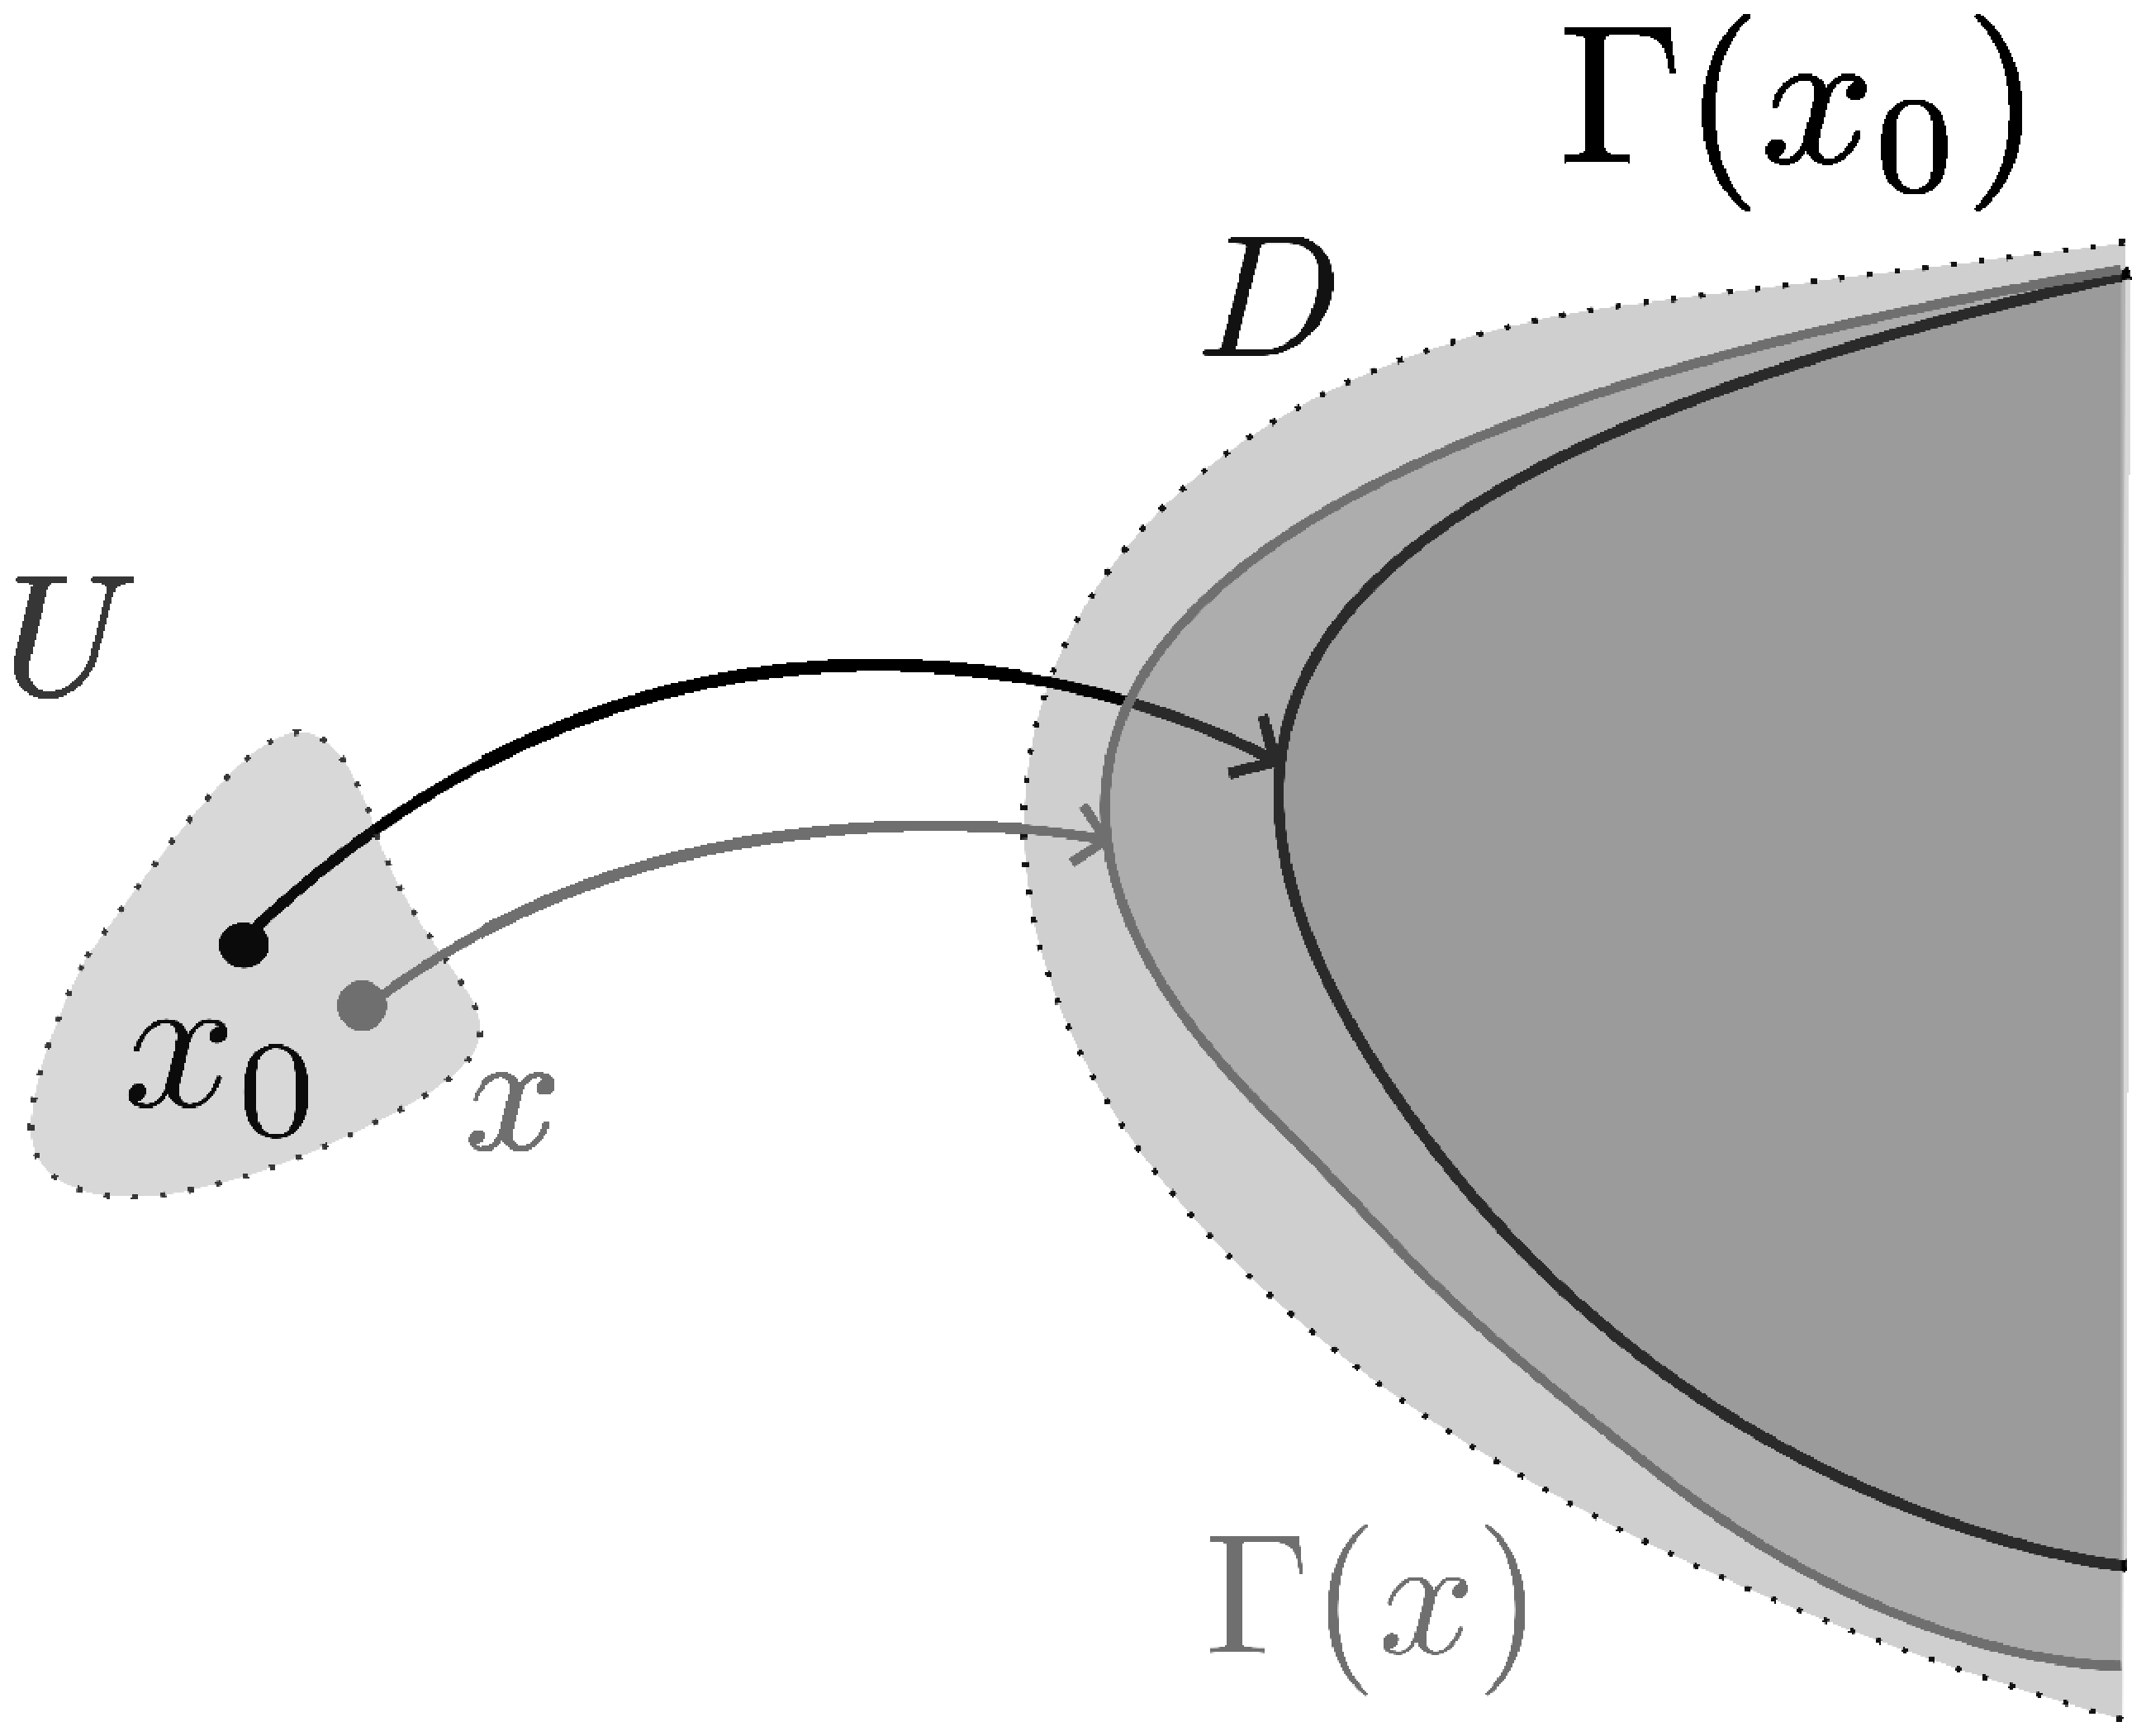
\includegraphics[keepaspectratio, scale=0.1]{figures/continuities/monochrome_upper_continuity.eps}
    \caption{upper continuity}
  \end{minipage}
  \hfill
  \begin{minipage}[b]{0.45\linewidth}
    \centering
    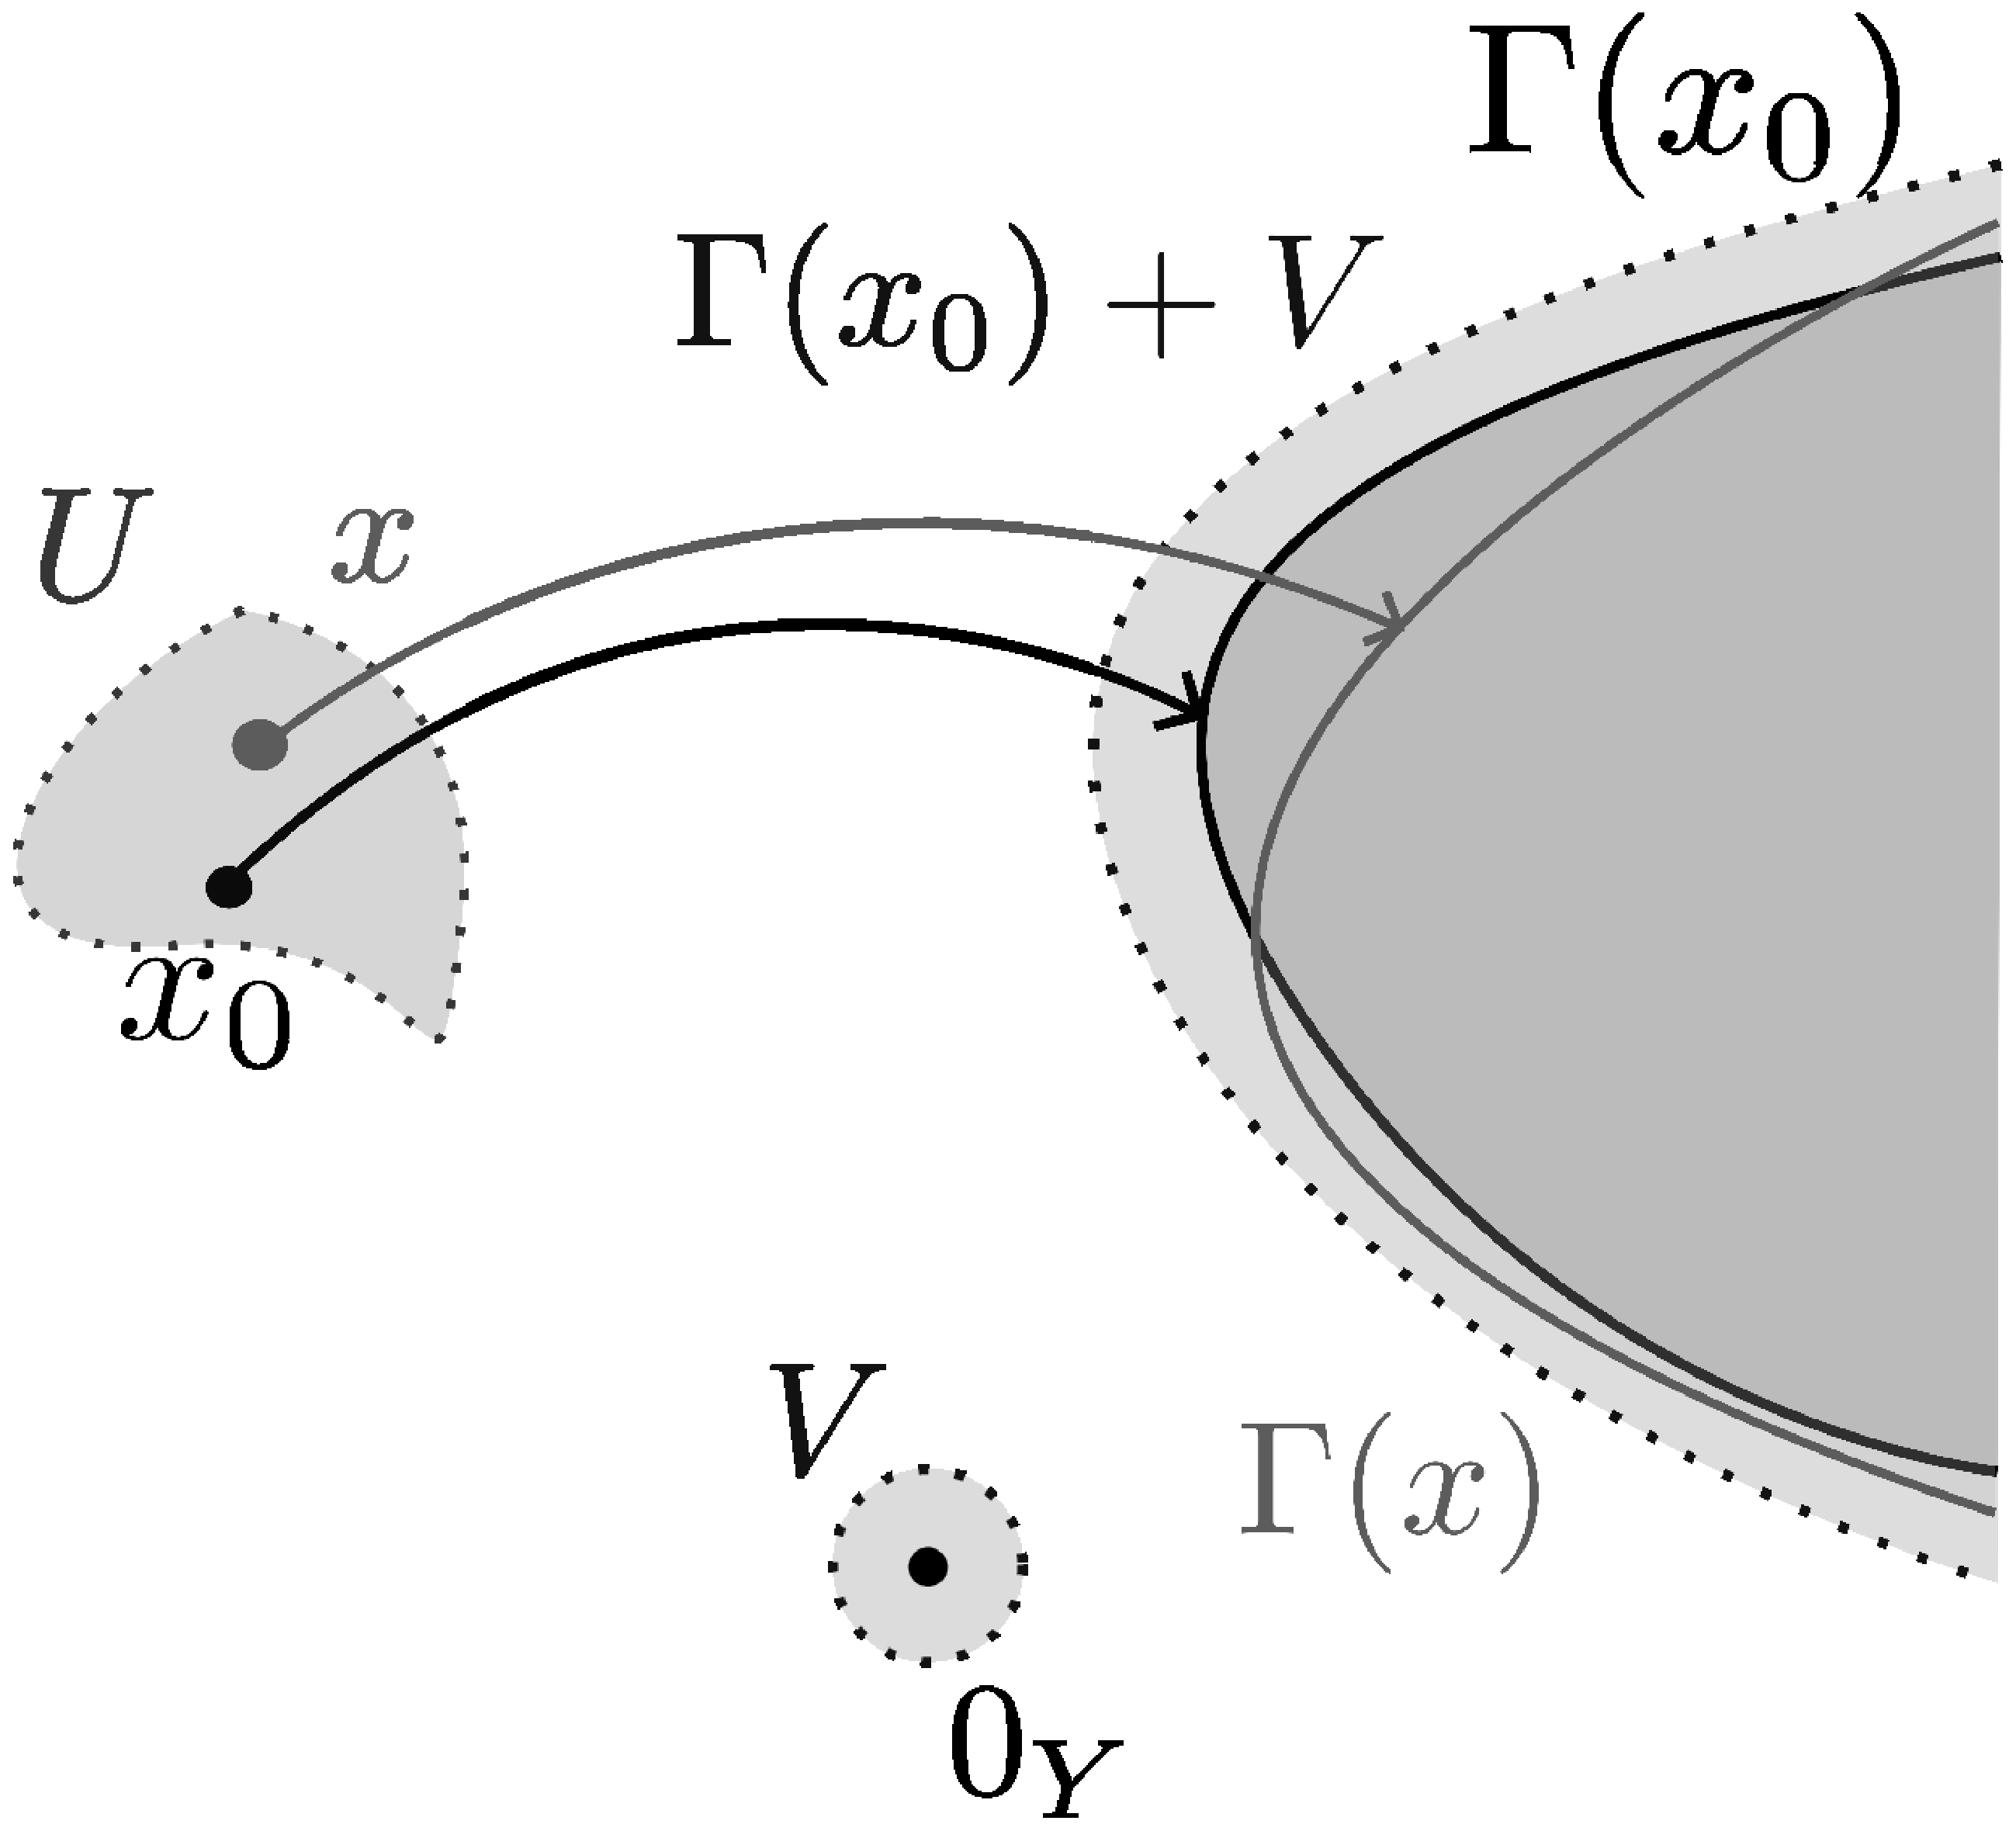
\includegraphics[keepaspectratio, scale=0.1]{figures/continuities/monochrome_h_upper_continuity.eps}
    \caption{Hausdorff upper continuity}
  \end{minipage}
  \hfill
  \mbox{}
\end{figure}

\section{\rm Main Results}

By the property between asymptotic cones and set valued mappings, we can study some continuities of set value mappings, from a nonempty convex set to the asymptotic cone. Let $C$ be a nonempty convex set in $\NDemenstionalRealEuclideanSpace$ and $\SetValudMapping (t) = \frac{C}{t}$ where $t>0$. Then, it does not always hold that $\SetValudMapping$ is upper continuous. Also, $\SetValudMapping$ is not always Hausdorff upper continuous. Considering the case of
\begin{equation}
  C = \{(x,y) \:|\: y \geq x^2\}, \notag
\end{equation}
$\SetValudMapping$ does not have the property of upper and Hausdorff upper continuities. In the paper, we only explain two continuities of set valued mappings, however, there are various continuities like lower continuity and Hausdorff lower continuity. As we study the relation between asymptotic cones and the continuities, the difference between a given set and the asymptotic cone can be expected. Thus, to conclude, we will research relationships between asymptotic cone and other continuities.

\begin{thebibliography}{9}
  \bibitem{Auslender03}
  A. Auslender and M. Teboulle, Asymptotic cones and functions in optimization and variational inequalities, Springer monographs in Mathematics, Springer-Verlag, New York, 2003.

  \bibitem{Tammer03}
  A. G\"{o}pfert, H. Riahi, C. Tammer, and C. Z\u{a}linescu, Variational methods in partially ordered spaces, vol. 17 of CMS Books in Mathematics, Springer-Verlag, New York, 2003.
  \end{thebibliography}
\end{document}
